\documentclass{standalone}
\usepackage{standalone}

\begin{document}
\chapter{Dataset}
\label{dataset}

One of the most challenging part of this work is to collect and process dataset. Thanks to pipilika.com\footnote{pipilika.com}o for providing us with their tagged dataset. We have also collected an open-source XML based Project by Prof. Dr. K. M. Azharul Hasan, Md. Mostafizur Rahman, Md. Abdulla-Al-Sun that contains a huge word tag-set \footnote{https://github.com/sunkuet02/BanglaPosTagger}..So we have two sets of data :
\begin{itemize}
    \item Tagged dataset by Pipilika.com
    \item XML word tagset
\end{itemize}
We will discuss them here in brief.
\section{Tagged dataset by Pipilika.com}
The dataset has been collected and processed by pipilika.com for their research purpose. We have collected them and processed them as we need. The dataset has 4943 lines and 47,594 words. The dataset has 12 classes :
\begin{itemize}
    \begin{itemize}
    \begin{multicols}{3}
    \item Adjective
    \item Adverb
    \item Conjunction
    \item Demonstrative
    \item Noun
    \item Particle
    \item Postposition
    \item Pronoun
    \item Punctuation
    \item Quantifier
    \item Residuals
    \item Verb
    \end{multicols}
    \end{itemize} 
\end{itemize} 

\begin{itemize}
    \item The initial dataset is a csv file with 47,594 rows and 5 columns titled sentence no, data, word, position, Tag. So each row contains the word, the corresponding tag and the position in the sentence.
    \begin{figure}[H]
    \centering
    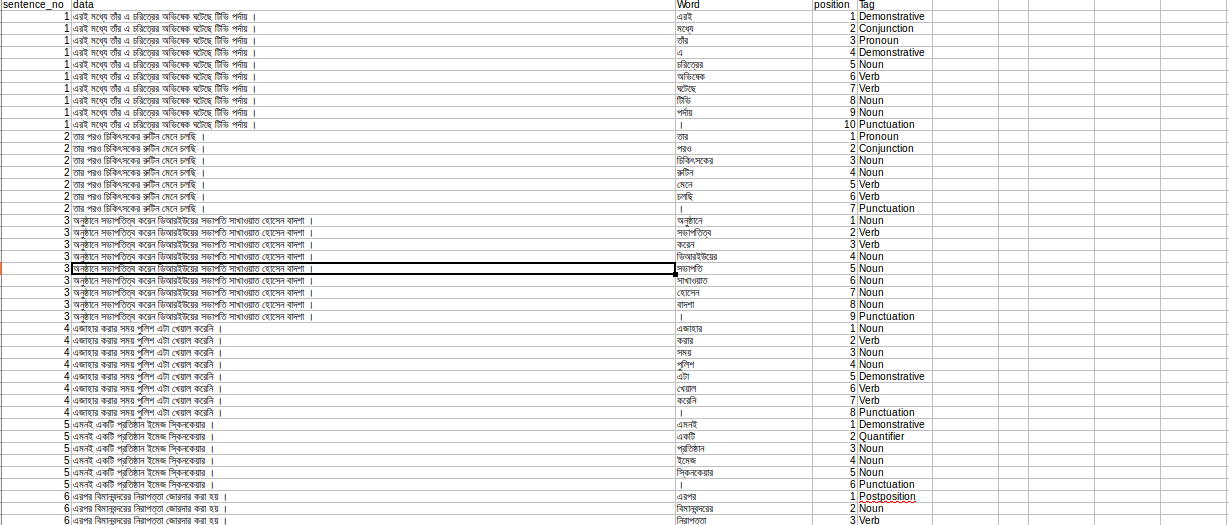
\includegraphics[width=1.0\columnwidth]{img/csvImage.png}
    \caption{Raw CSV dataset}
    \label{csv1}
    \end{figure}
\end{itemize}

\begin{itemize}
    \item we have processed raw dataset and got lines of words with their corresponding tag. There are 4953 lines in the dataset.
    \begin{figure}[H]
    \centering
    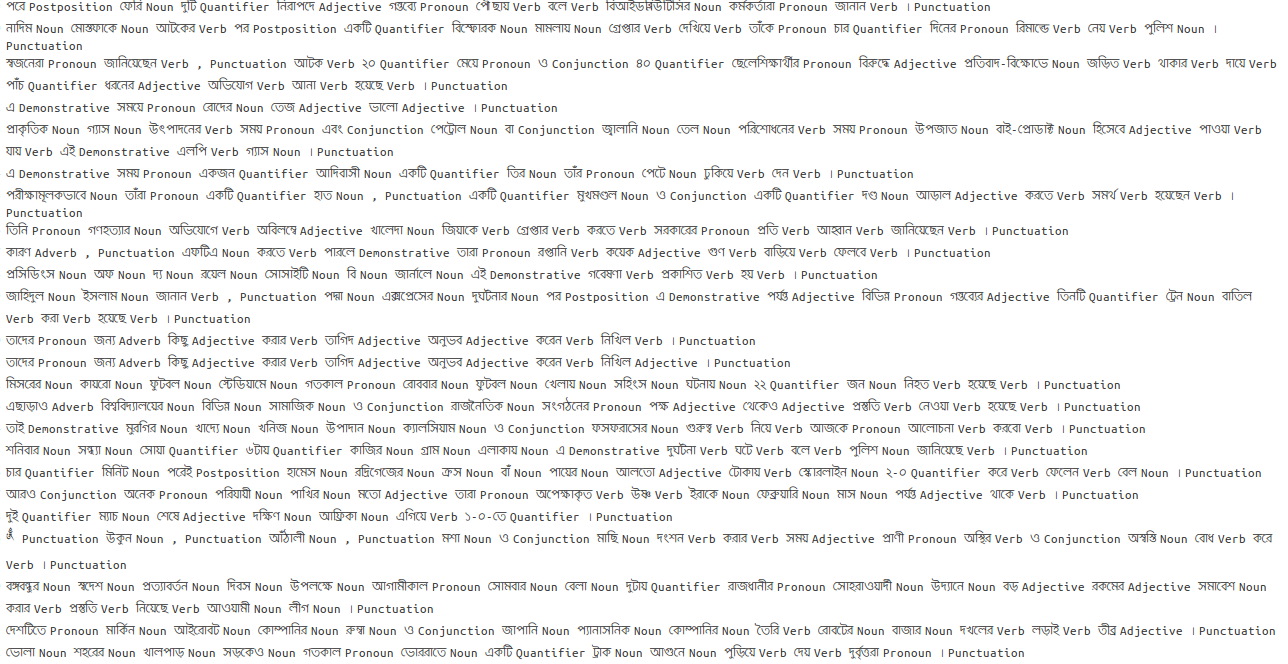
\includegraphics[width=1.0\columnwidth]{img/linesFinal.png}
    \caption{Lines with tags}
    \label{linesFinal}
    \end{figure}
\end{itemize}
\begin{itemize}
    \item Then we have created a file containing the frequency of each word being the Parts of Speech. From this file, we get 11528 different words and their frequency of being each Parts of Speech in the dataset.
     \begin{figure}[H]
    \centering
    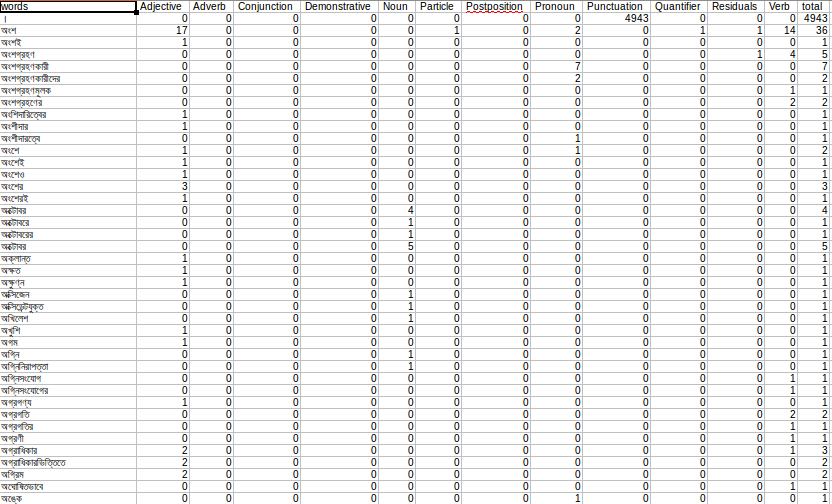
\includegraphics[width=1.0\columnwidth]{img/worg-tag-frequency.png}
    \caption{word tag frequency}
    \label{wordtagfrequency}
    \end{figure}
\end{itemize}

\section{XML word tagset}
We needed a huge corpus of words with their tag frequency. Unfortunately, we could not collect or create this huge corpus. So we have taken the open-source XML based Project by Prof. Dr. K. M. Azharul Hasan, Md. Mostafizur Rahman, Md. Abdulla-Al-Sun. This XML file contains 1,12,382 word with corresponding tag\footnote{https://github.com/sunkuet02/BanglaPosTagger}.
\begin{itemize}
    \item The XML dataset was in the form presented in the figure \ref{sd1}
    \begin{figure}[h!]
    \centering
    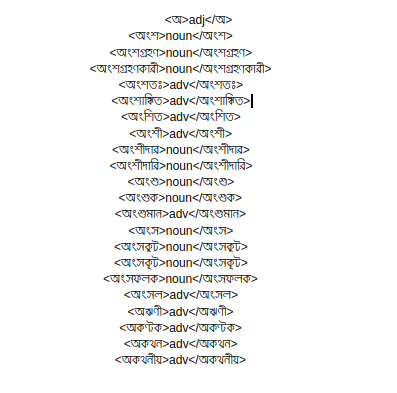
\includegraphics[width=1.0\columnwidth]{img/xml.png}
    \caption{XML-based tagset sample}
    \label{sd1}
    \end{figure}
\end{itemize}
\begin{itemize}
    \item The word Dictionary was in XML form, so we had to convert it into text form where the first word of a line contains the word and the second one defines the respective POS.\\
    \begin{figure}[h!]
    \centering
    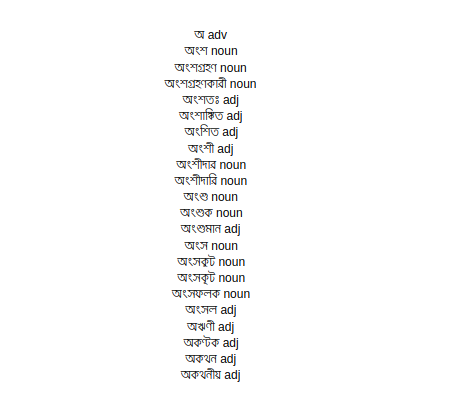
\includegraphics[width=1.0\columnwidth]{img/dict.png}
    \caption{Processed Tagset Sample}
    \label{sd3}
    \end{figure}
    \\
    The figure \ref{sd3} shows the processed samples in the figure \ref{sd1}.
\end{itemize}
\begin{itemize}
    \item our dataset is divided into 80:20 for training and test set. The training set contains 3461 lines and the test set contains 1483 lines. We have also processed the training lines suitable for our training features. For each word, we have created a line containing the probabilistic feature of it’s previous and next two words and it’s own feature. An example is shown in \ref{trainset}
    \begin{figure}[h!]
    \centering
    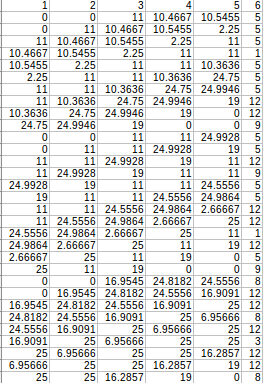
\includegraphics[width=1.0\columnwidth]{img/trainset.png}
    \caption{Training Features}
    \label{trainset}
    \end{figure}
\end{itemize}





\end{document}